\documentclass[10pt,fleqn]{beamer}

\usepackage[portuges,brazilian]{babel}
\usepackage[T1]{fontenc}
\usepackage[utf8]{inputenc}

\usepackage{multirow} % To merge cels horizontaly

\usepackage{multicol} % para utilizar ambiente "multicols"
\usepackage{pdfpages} % para incluir paginas de documentos PDFs
\usepackage{color, amsmath}
\usepackage{subfigure}
\usepackage{graphicx} % para incluir figuras
\usepackage[ruled,longend]{algorithm2e} % para escrever algoritmos
\usepackage{ulem}       % para trocar a fonte?

\definecolor{defblue}{rgb}{0.2, 0.2, 0.7}
\definecolor{defred}{rgb}{0.4, 0.0, 0.0}
\definecolor{defgreen}{rgb}{0.0, 0.4, 0.0}

\definecolor{ninfagreen}{rgb}{0.168, 0.541, 0.569} % changed this

% Set left ident of equations
\setlength{\mathindent}{4pt}

\newcommand{\mydef}[1]{{\vspace{8pt} \large \color{defblue} #1}}
\newcommand{\myred}[1]{{\bf \color{defred} #1}}
\newcommand{\mygreen}[1]{{\bf \color{defgreen} #1}}

\renewcommand{\rmdefault}{put} % Utopia Font
\renewcommand{\sfdefault}{put} % Utopia Font
\renewcommand{\emph}[1]{ {\bf #1} }

% Scale Equations
\newcommand*{\Scale}[2][4]{\scalebox{#1}{$#2$}}%

\newcommand{\litem}[1]{
  \item{#1 \vspace{9pt}}
}

%\usetheme{Berkeley}
%\usetheme{Hannover}
%\usetheme{Marcos}
%\usetheme{default}
\usetheme{Boadilla}
%\usetheme{Pittsburgh}

%\useinnertheme{rectangles}
%\useoutertheme{tree}
%\setbeamercolor{separation line}{use=structure,bg=structure.fg!50!bg}

%\usecolortheme{dolphin}
%\usecolortheme{seahorse}

\beamertemplatenavigationsymbolsempty

% Escrita dos algoritmos
\SetKwInput{KwIn}{Entrada}
\SetKwInput{KwOut}{Saída}
\SetKwFor{While}{enquanto}{faça:}{fim}
\SetKwFor{For}{para}{faça:}{fim}
\SetKwBlock{Begin}{início}{fim}
\SetKwIF{If}{ElseIf}{Else}{se}{então}{senão se}{senão}{fim}

\newcommand{\bigbullet}{\,\begin{picture}(-1,1)(-1,-2)\circle*{5}\end{picture}\ }
\newcommand{\termo}[1]{\textbf{#1}}
\newcommand{\titulo}[1]{\centering \LARGE \vfill \textcolor{defblue}{\textbf{#1}} \vfill }

\newcommand{\chamada}[1]{
  \textcolor{ninfagreen}{\textbf{#1}}
  \vspace{10pt}
}

%\title{Um Estudo da Eficiência da Autocentralidade no Problema de Isomorfismo de Grafos}
\title[]{O algoritmo Nemhauser-Ullmann para o problema de mochila multidimensional}
\subtitle{}
\author{Marcos Daniel Baroni}
\institute[NINFA]{}
\date[Vitória, 15/01/2015]{Vitória, 15 de janeiro de 2015}
\subject{}

% Figura de fundo
\setbeamercolor{background canvas}{bg=white}
\setbeamertemplate{background}{\includegraphics[width=\paperwidth,bb=0 0 1036 777]{figs/fundo.png}}

% Posição dos títulos dos slides
\addtobeamertemplate{frametitle}{\vskip 2.5ex }{}
\addtobeamertemplate{frametitle}{\bf }{}

\begin{document}

\definecolor{beamer@blendedblue}{rgb}{0.168, 0.541, 0.569} % changed this

%\setbeamercolor{normal text}{fg=black,bg=white}
%\setbeamercolor{alerted text}{fg=red}
%\setbeamercolor{example text}{fg=green!50!black}

%\setbeamercolor{structure}{fg=beamer@blendedblue}

%\setbeamercolor{background canvas}{parent=normal text}
%\setbeamercolor{background}{parent=background canvas}

%\setbeamercolor{palette primary}{fg=yellow,bg=yellow} % changed this
%\setbeamercolor{palette secondary}{use=structure,fg=structure.fg!100!green} % changed this
%\setbeamercolor{palette tertiary}{use=structure,fg=structure.fg!100!green} % changed this

\begin{frame}
  \titlepage
\end{frame}

\begin{frame}
  \frametitle{Sumário}
  \begin{itemize}
    \litem{Introdução}
    \litem{O problema da Mochila (Multidimensional)}
    \litem{O Algoritmo de Nemhauser-Ullmann para o MKP}
    \begin{itemize}
      \litem{O Conceito de Soluções Dominantes}
      \litem{O Algoritmo para o KP}
      \litem{Adaptação do Conceito para o MKP}
    \end{itemize}
    \litem{Testes Computacionais}
  \end{itemize}
\end{frame}

\section{Introdução}

\begin{frame}
  \frametitle{O Problema da Mochila} % versão padrão
  \framesubtitle{\textit{Knapsack Problem}}
  Utilizar a mochila para carregar o maior valor possível, respeitando a sua
  capacidade.
  \begin{columns}[T]
    % Primeira coluna
	  \begin{column}{.5\textwidth}
      \begin{block}{Modelagem matemática}
	    { \footnotesize
        \begin{align*}
          \textrm{maximizar} \quad
		  	& z = \sum_{j=1}^n p_j x_j \\
          \textrm{sujeito a} \quad
		  	& \sum_{j=1}^n w_{j}x_j \leq b \\
            & {x_j \in \{0,1\}, \quad j=1,\cdots,n.}
        \end{align*}
		}
      \end{block}
    \end{column}
    % Segunda coluna
    \begin{column}{.5\textwidth}
	  \begin{center}
        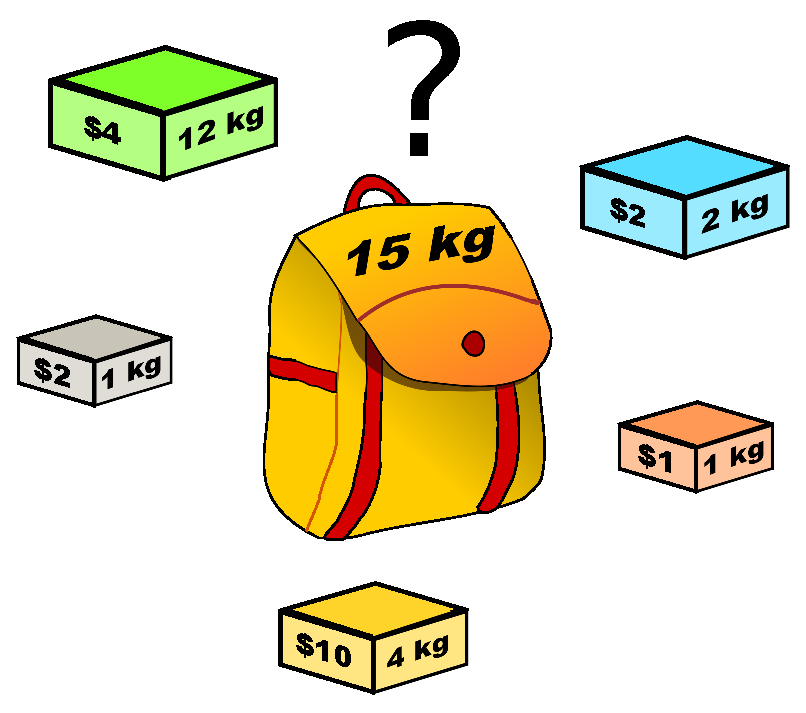
\includegraphics[scale=0.3]{figs/knapsack}
	  \end{center}
    \end{column}
  \end{columns}
\end{frame}

\begin{frame}
  \frametitle{O Problema da Mochila Multidimensional}
  A \textit{mochila} agora possui mais de uma capacidade (dimensão).
  \begin{minipage}{6cm}
    \begin{block}{Modelagem matemática}
    { \footnotesize
       \begin{align*}
         \textrm{maximizar}
           \quad & z = \sum_{j=1}^n p_j x_j \\
         \textrm{sujeito a}
 	        \quad & \sum_{j=1}^n w_{ij}x_j \leq b_i, \quad i=1,\cdots,m, \\
                & x_j \in \{0,1\}, \quad j=1,\cdots,n.
       \end{align*}
	}
	\end{block}
    \end{minipage}
\end{frame}

\begin{frame}
  \frametitle{Soluções dominantes para o KP}
  \begin{minipage}{10cm}
    \begin{block}{Solução dominante}
    Um subconjunto $S \subseteq [n]$ com peso $w(S) = \sum_{i \in S} w_i$ e lucro 
	  $p(S) = \sum_{i \in S} p_i$ \emph{domina} sobre um outro subconjunto
	  $T \subseteq [n]$ se $w(S) \leqslant w(T)$ e $p(S) \geqslant p(T)$.
	\end{block}
  \end{minipage}
\end{frame}

\begin{frame}
  \frametitle{Soluções dominantes para o KP}
	\begin{center}
      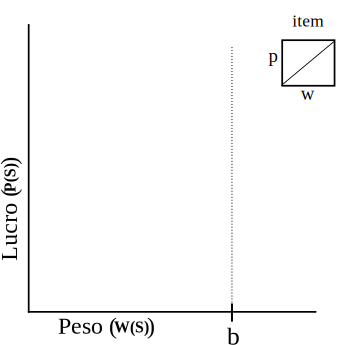
\includegraphics[scale=0.7]{figs/axis-1dim}
	\end{center}
\end{frame}


\begin{frame}
  \frametitle{O Algoritmo de Nemhauser-Ullmann}
\begin{algorithm}[H]
 \SetKwInOut{Input}{Input}
 \SetKwInOut{Output}{Output}
 \Input{Instancia do KP}
 \Output{Lista $S(n)$ de todos as soluções dominantes}
 $S(0) \leftarrow \emptyset $\;
 \For{$i\leftarrow 1$ \KwTo $n$}{
   $S'(i) \leftarrow S(i-1)\; \cup \big\{ s \cup \{i\} \,\big|\, s \in S(i-1)\big\}$\;
   $S(i) \leftarrow \big\{ s \in S'(i) \,\big|\, \mathsf{dominates}\big(s, S'(i)\big) \big\}$\;
 }
 \caption{O Algoritmo de Nemhauser-Ullmann para o KP}
 \label{alg:nu}
\end{algorithm}
\end{frame}

\begin{frame}
  \frametitle{O Algoritmo de Nemhauser-Ullmann}
  \begin{figure}[h]
    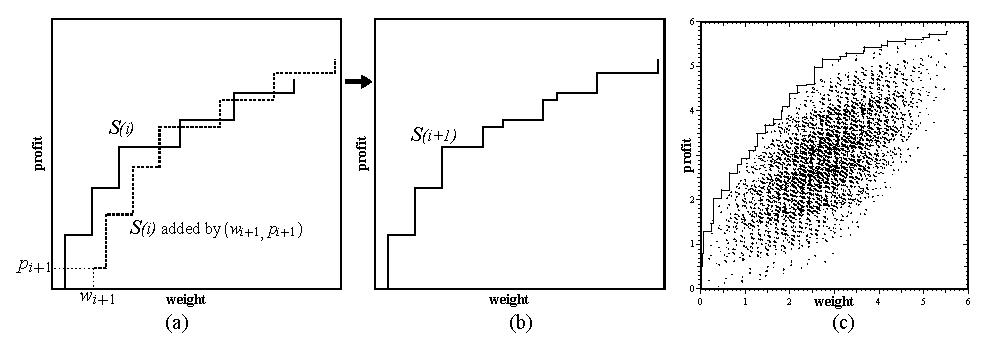
\includegraphics[width=\textwidth]{figs/pareto}
    \caption{Representação gráfica das soluções dominantes
    (a) num passo intermediário $S(i)$, (b) em uma próxima solução $S(i+1)$ e
    (c) numa solução ótima (final).}
    \label{fig:pareto}
  \end{figure}
\end{frame}

\begin{frame}
  \frametitle{O Algoritmo de Nemhauser-Ullmann para o MKP}
  \begin{minipage}{12cm}
    \begin{block}{Solução dominante (para o MKP)}
    Um subconjunto $S \subseteq [n]$ com pesos $w_j(S) = \sum_{i \in S} w_{ji}, j = 1, \ldots, m$ e lucro 
	  $p(S) = \sum_{i \in S} p_i$ \emph{domina} sobre um outro subconjunto
	  $T \subseteq [n]$ se $w_j(S) \leqslant w_j(T), \forall j = 1, \ldots, m$ e $p(S) \geqslant p(T)$.
	\end{block}
  \end{minipage}
\end{frame}

\begin{frame}
  \frametitle{Soluções dominantes para o MKP}
	\begin{center}
      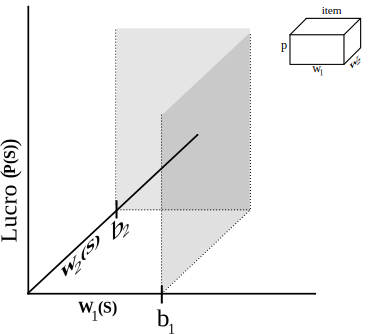
\includegraphics[scale=0.7]{figs/axis-2dim}
	\end{center}
\end{frame}


\begin{frame}
  \frametitle{Testes computacionais}
	\begin{center}
      \includegraphics[scale=0.75]{graficos/results}
	\end{center}
\end{frame}

\begin{frame}
  \frametitle{Testes computacionais}
  \begin{figure}
	\begin{center}
      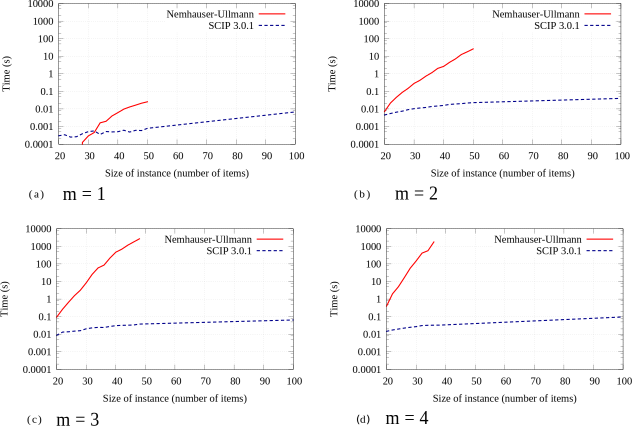
\includegraphics[scale=0.5]{graficos/scip}
	\end{center}
  \caption{\scriptsize Tempo médio de execução para resolver instancias do MKP
  utilizando o algoritmo de Nemhauser-Ullmann e o SCIP solver para várias dimensões.
  }
  \end{figure}
\end{frame}


\begin{frame}
  \frametitle{Referências Bibliográficas}
  \nocite{weingartner1967methods}
  \nocite{nemhauser1969discrete}
  \nocite{beier2003random}
  \nocite{beier2006experimental}
  \bibliographystyle{abbrv}
  { \small
  \bibliography{../../../refs}
  }
\end{frame}

\end{document}
